\chapter{Review on mass spectrometry (\ac{MS}) and shotgun proteomics}
\label{chap:mass_spec}


The main source of data in proteomics is Mass Spectrometry (\ac{MS}). However, different approaches to how this technique is used make for two paradigms in proteomics analysis: top-down and bottom-up \cite{Joshi2016}. In the top-down paradigm, intact proteins are directly used for the analysis \cite{Sinitcyn2018}. In the bottom-up paradigm (see figure \ref{fig:proteomics_overview}), the proteins are first cleaved into smaller parts, and these parts are then used for identification, characterization, and quantification. These smaller parts are peptides \cite{Barsnes2008}, consisting of around 10 chained aminoacids. Such peptides acquire physicochemical properties fitting the requirements of the downstream analytical methods, mainly the mass spectrometer (MS), which performs the data acquisition. The bottom-up paradigm is most often used because peptides are much more suitable to analysis by mass spectrometry, as illustrated in section \ref{subsec:the_detector}. This review will focus on the Data-Dependent Acquisition (\ac{DDA} approach within bottom-up proteomics, which currently is the most frequent workflow in proteomics \cite{Sinitcyn2018}. In this approach, the equipment is configured for the analysis of one peptide at a time, with the drawback of being biased for the most abundant peptides.

\begin{figure}[!h]
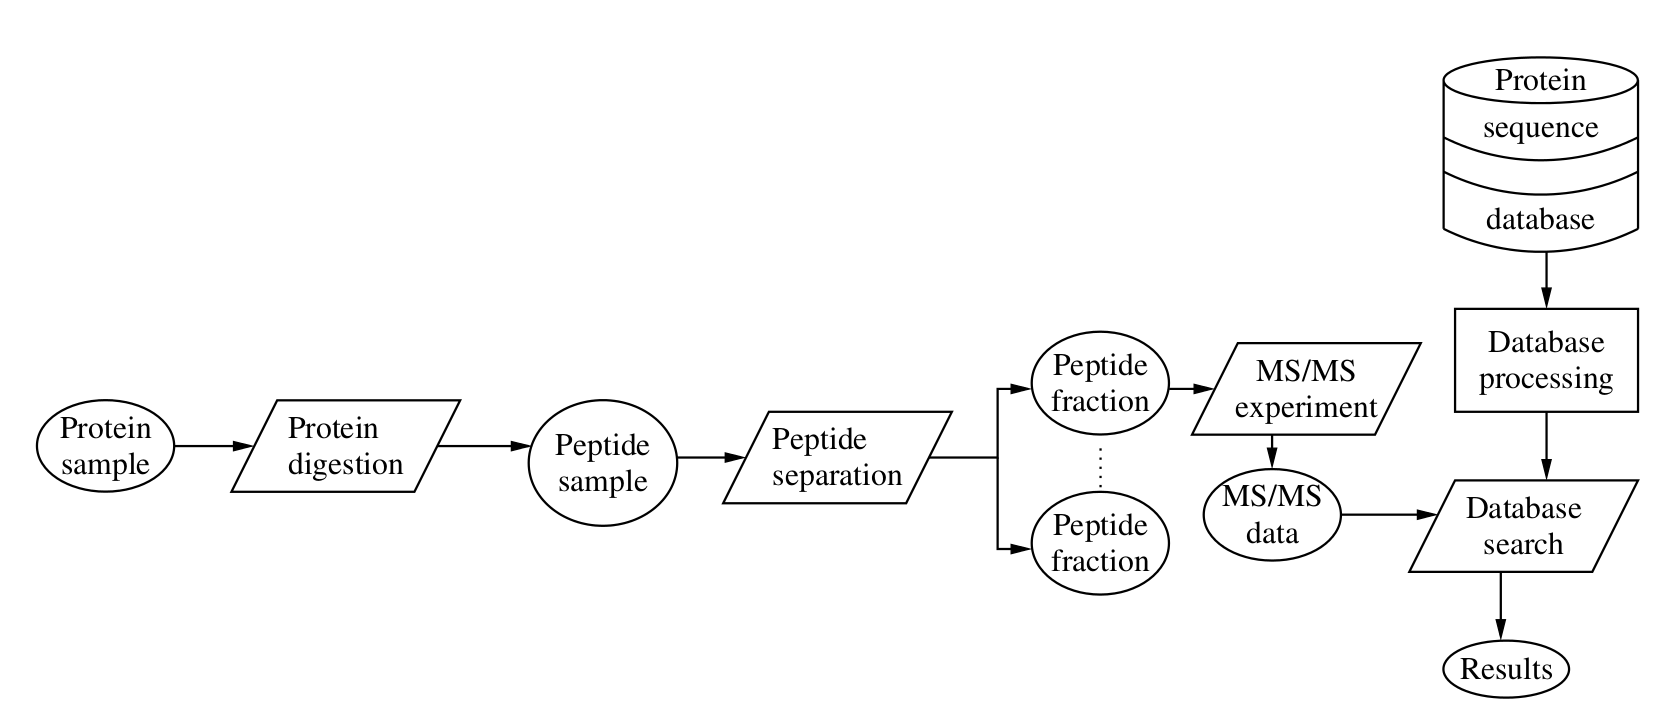
\includegraphics[width=\textwidth]{proteomics_skema_book}
\caption[Bottom-up proteomics analysis]{Diagram over a standard bottom-up proteomics analysis. Figure 1.3 from \cite{Barsnes2008}.}
\label{fig:proteomics_overview}
\end{figure}

\ac{MS} is performed by means of a mass spectrometer, an ensemble of pieces of equipment that can acquire mass measurements for eventually thousands of analytes. A detailed explanation of the sample processing required prior to \ac{MS} is given in section \ref{sec:sample_processing}, while an overview on mass spectrometers is given in section \ref{sec:the_mass_spectrometer}. The result of the MS analysis is a dataset that, with adequate computational analysis tools, is enough to perform the inference steps required to gather knowledge about the original protein composition in a sample. These inference steps can be condensed to the peptide and protein inference problems, explained in section \ref{sec:inference}. A third computational challenge needs to be solved if quantitative, and not just qualitative information, has to be gained from the experiment. This is the quantification problem, explained in section \ref{sec:quantification}.

A summary of the bottom-up approach MS analytical pipeline is provided in the rest of the chapter. It can be divided into two main steps:

\begin{enumerate}

\item \ac{MS} analysis and data generation. Sections \ref{sec:sample_processing} to \ref{sec:tandem_ms_workflow}.

\item Computational analysis of data. Sections \ref{sec:search_engines} to \ref{sec:quantification}.

\end{enumerate}

\section{Sample processing}

Prior to its introduction in the mass spectrometer for shotgun proteomics studies, a protein sample (I) is cleaved into peptides and (II) these peptides are separated by means of some physicochemical properties. This way, the analytical equipment works with one peptide at a time.

\label{sec:sample_processing}

\begin{figure}[!h]
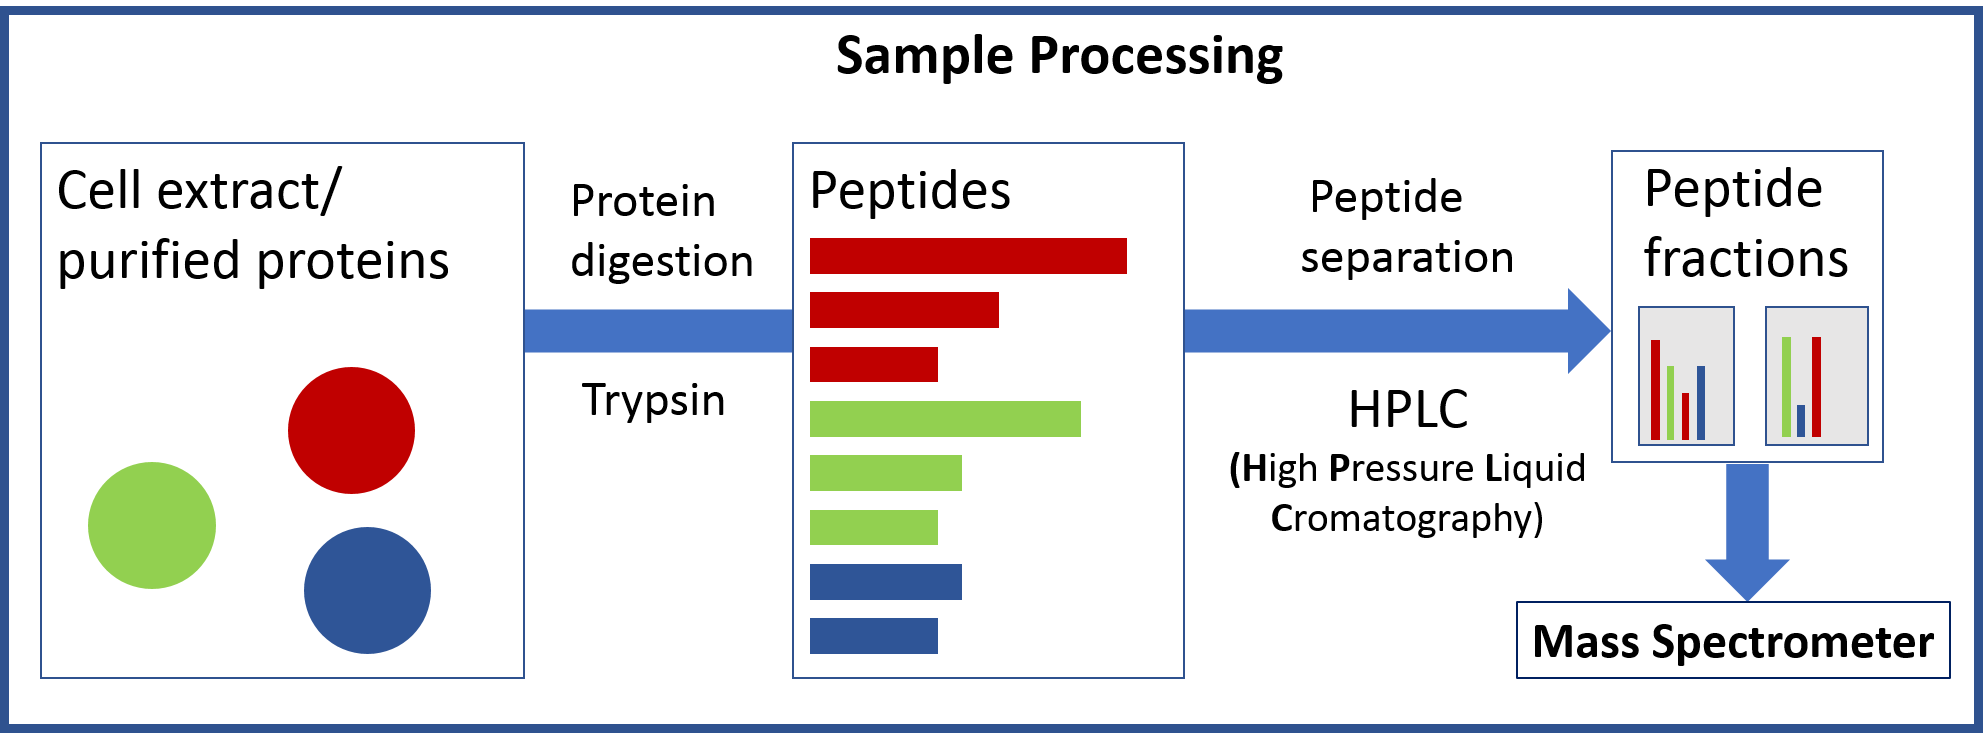
\includegraphics[width=\textwidth]{sample_processing}
\caption[Sample processing summary]{Diagram of the sample processing step prior to mass spectrometry analysis. First, proteins are denatured and digested with a specific protease like Trypsin. This yields a peptide mix that is separated into peptide fractions that can be introduced in the mass spectrometer.}
\label{fig:sample_processing}
\end{figure}

\subsection{Protein digestion}
\label{subsec:protein_digestion}

An \ac{MS} experiment starts with the generation of a protein sample from the biological system of interest. Proteins are then denatured  so as to remove bias due to the divergent properties acquired by their folded state. Then, proteins are subjected to digestion with specific proteases i.e protein-cutting molecules, which cut the aminoacidic chains following a predictable pattern. Trypsin is the most frequently used protease. It cuts peptidic bonds whenever a positively charged residue, either lysine (K) or arginine (R), lies on the carboxyl side of the peptidic bond. Since roughly 2/20 residues are either R or K, the average peptide length is 10 residues, as mentioned before. As demonstrated in section \ref{subsec:the_detector}, this length distribution is fitted to the resolution of the MS analyzer. Moreover, for as much as R and K are positively charged aminoacids (see figure \ref{fig:aminoacids}), the resulting peptide is guaranteed, in most cases, to be able to capture at least one charge, which is key in the \ac{MS} workflow as described in section \ref{sec:the_mass_spectrometer}. All of these properties combined, together with its low price, makes Trypsin the protease of choice in this step for most cases.

Even though proteases are very specific, the cleaving process is far from perfect, as there could be: \cite{Barsnes2008}
%COMPUTATIONAL METHODS 3.2

\begin{enumerate}

\item Missed cleavages.

\item Unsuspected cleavages during the maturation/life cycle of the protein.

\item Unexpected cleavages occurring in the wet-lab procedure of the proteolytic treatment.

\item Naturally occurring, intentionally or unintentionally induced chemical modifications.

\end{enumerate}

Missed cleavages can happen due to steric impediments or the presence of specific aminoacids that can weaken the enzyme\textquotesingle s function \cite{Siepen2007}. This is the case of Trypsin whenever the residue on the other side of the peptidic bond is a proline. Altogether, a variability is created in the cleavage process that, though limited, needs to be taken care of in downstream analysis, as it could introduce biases in peptide observability.

The result of this process is a complex mix of peptides, made up by hundreds or thousands of different molecules, following a length distribution given by the cleavage sites frequency and each protein\textquotesingle s aminoacidic composition. A peptide separation step is required before introducing the sample in the spectrometer.

\subsection{Peptide separation}
\label{subsec:peptide_separation}

If presented with the problem of analyzing a mixture of peptides, the capacities of mass spectrometers are easily overwhelmed by a too complex mixture, resulting in the analysis of only a minor part of the total protein of the sample \cite{Barsnes2008}. This can be surmounted by analyzing one peptide in the sample at a time. The required sample separation is achieved by High-Performance Liquid Chromatography (\ac{HPLC}) methods, like reverse phase chromatography (separating on hydrophobicity) and strong cation exchange chromatography (separating on isoelectric point) \cite{Barsnes2008}.

%CITE 4.2 computational methods.
During \ac{HPLC}, the peptide mix is loaded into a column containing a stationary and a solid phase. These phases create an environment where peptides interact with the column differently based on their physico-chemical properties, set by the nature of the phases. The output of the column, called elute, will consist of subsets or fractions of peptides leaving the column at different retention times (\ac{RT}) i.e. the amount of time passed before the peptide is observed in the mass spectrometer. Therefore, the input to the spectrometer will consist of few peptides at any given time.

\section{The mass spectrometer}
\label{sec:the_mass_spectrometer}

The mass spectrometer is the ensemble of pieces of equipment analyzing peptides like those generated following the workflow described in sections \ref{sec:sample_processing} and \ref{subsec:peptide_separation}. It consists of three main parts: an ion source, a mass analyzer, and a detector (see figure \ref{fig:mass_spectrometer}) \cite{Barsnes2008}.

\begin{figure}[!h]
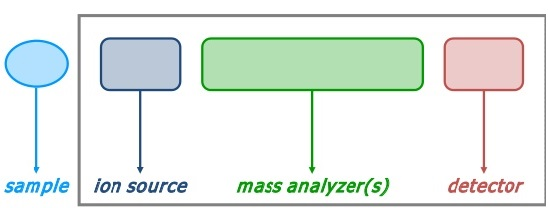
\includegraphics[width=\textwidth]{mass_spectrometer}
\caption[Mass spectrometer diagram]{Schematic view of a mass spectrometer. Taken from \href{https://www.slideshare.net/joachimjacob/bits-introduction-to-mass-spec-data-generation}{https://www.slideshare.net/joachimjacob/bits-introduction-to-mass-spec-data-generation}.}
\label{fig:mass_spectrometer}
\end{figure}
%
%\footnotetext{\href{https://www.slideshare.net/joachimjacob/bits-introduction-to-mass-spec-data-generation}{https://www.slideshare.net/joachimjacob/bits-introduction-to-mass-spec-data-generation}}
%\stepcounter{footnote}

\subsection{The ion source}
\label{subsec:the_ion_source}

All mass spectrometers exploit the physical properties of mass and electric charge exhibited by the analyzed components. Ionization of the analytes is absolutely essential prior to any measurement, as analytes left uncharged will be invisible to the equipment.

%CITE 5.1 COMPUTATIONAL METHODS

This step is performed in the ion source \cite{Barsnes2008}. The most frequent ionization methods in proteomics are Matrix-Assisted Laser Desorption-Ionization (\ac{MALDI}) and Electro Spray Ionization (\ac{ESI}) \cite{Mirzaei2016}. Most peptides ionized by \ac{MALDI} will acquire a single charge, whereas \ac{ESI} can provide multiple charges (+2, +3, etc) \cite{Joshi2016}. Thus, the charge exhibited by an ion is not obvious when produced via \ac{ESI}. Moreover, \ac{ESI} can be run online with the right robotic equipment, while \ac{MALDI} demands waiting time for vacuum generation. Finally, due to the chemical nature of the matrix components, MALDI ionizes more easily peptides containing aminoacids featuring aromatic rings (PYW) \cite{Hessling2013}, thus introducing a bias \cite{Hessling2013}, whereas bias in \ac{ESI} is less predictable. All the sources of bias introduced during ionization cause the competitive ionization problem \cite{Zhang2009} \cite{Tang2004}.

The acquired charge yields a mass/charge (\ac{m/z}) ratio, a property that is applied in the downstream component separation and measurement steps. It is measured in $\frac{Da}{e}$ (Dalton over elementary charge), sometimes referred to as Th (Thomson).

\subsection{The mass analyzer}
\label{subsec:the_mass_analyzer}

The plethora of ion separation methods is reflected upon the range of different analyzers available, mainly Time Of Flight (\ac{TOF}), Ion Trap (\ac{IT}) and Quadrupole (\ac{Q}). These apply different principles to perform the same task: separation (analysis) of the ion mix by the \ac{m/z} ratio.

Moreover, two other analyzers exist which combine mass analysis with intensity measurement. These are Fourier Transform Ion Cyclotron Resonance (\ac{FT-ICR}) and Orbitrap. They both register cyclotron resonance frequencies that are Fourier transformed into the spectrum space. Remarkably, \ac{FT-ICR} exhibits great resolving power, at the cost of high maintenance costs and difficult operation \cite{Barsnes2008}. 

\subsection{The detector}
\label{subsec:the_detector}

Detectors measure the intensity of an incoming ion signal. The ion\textquotesingle s \ac{m/z} ratio is known thanks to the previous mass analysis step. Run on enough \ac{m/z} ratios, the detector can produce an \ac{MS} spectrum, which shows the ion current intensity over an \ac{m/z} range. Some topics in signal detection in \ac{MS} need to be discussed.

On the one hand, the precision of the signal measurement is given by its mass resolution. It is conventionally defined as the closest distinguishable separation between two peaks of equal height and width \cite{Marshall2013}. The resolution decreases as the \ac{m/z} ratio increases because small increments in the \ac{m/z} ratio become negligible at high \ac{m/z} ratios. This is one of the reasons why proteins are better fit for analysis when digested into peptides, as \ac{m/z} are reduced, thus increasing the mass resolution.

On the other hand, due to the natural occurrence of isotopes, particularly \ce{^{13}_{}C}, the same peptide will induce the measurement of several signals with very close \ac{m/z} values. They constitute the isotopic envelope of the ion (see figure \ref{fig:envelope}) \cite{Mirzaei2016}, and represent the signal created by peptides containing an increasing number of \ce{^{13}_{}C} atoms or other naturally occurring isotopes. Every time a \ce{^{12}_{}C} is replaced by \ce{^{13}_{}C}, the molecule\textquotesingle s mass increases by 1 Da. Even though the natural abundance of \ce{^{13}_{}C} is 1.1 \%, the sheer number of carbon atoms in a peptide makes it likely that at least one or even more carbon atoms will be \ce{^{13}_{}C}, eventually driving the pure \ce{^{12}_{}C} signal to comparatively small intensity values, and down to intensities below the background noise. Such event can be problematic if it entails that the \ce{^{13}_{}C} peak is confused for the \ce{^{12}_{}C} peak.

\begin{figure}[!h]
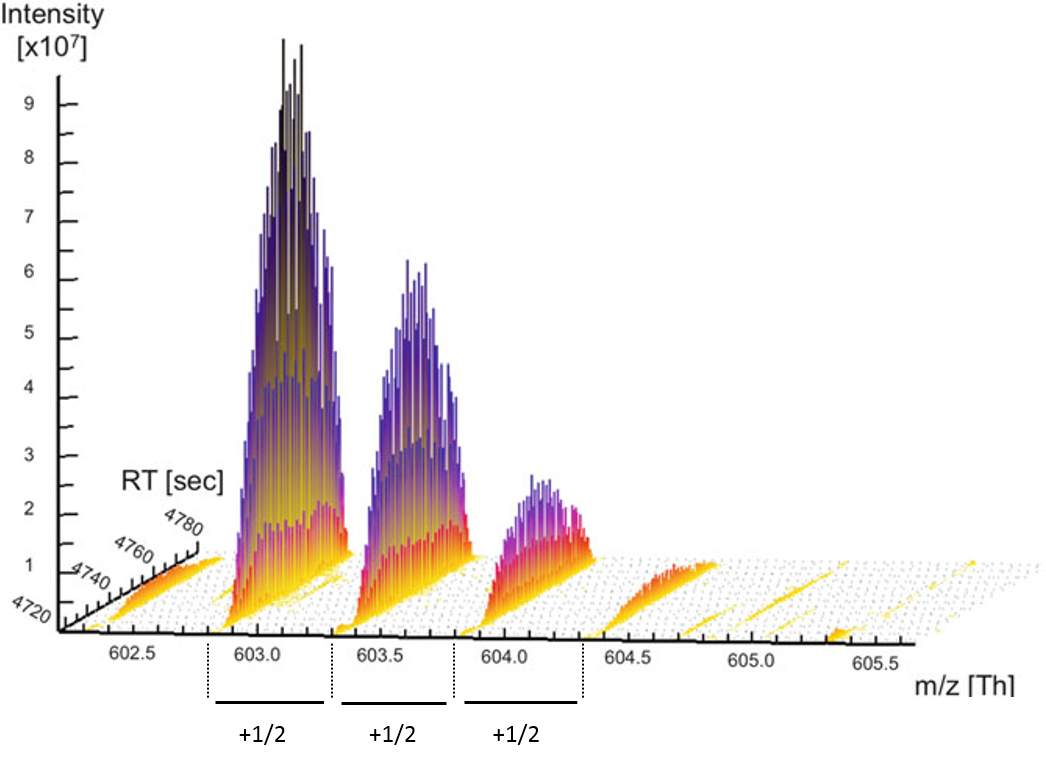
\includegraphics[width=\textwidth]{envelope}
\caption[Isotopic envelope]{A doubly charged isotopic envelope with its monoisotopic ion measured at 602.8 Th. Each peak in the envelope is separated by 0.5 Th. This is explained by the peptide having 2 positive charges that make every extra Da in the ion mass account for 1/2 extra Th. Adapted from \cite{Mirzaei2016}.}
\label{fig:envelope}
\end{figure}


The resolution achieved by modern equipment allows for the distinction of each individual signal in most isotopic envelopes. Remarkably, the separation across peaks in the envelope can be used to infer the charge of the peptide with the following expression (see equation \ref{eq:envelope}):

\begin{equation}\label{eq:envelope}
m/z = \frac{(m + z × H^+)}{z} \text{for \textit{z}} \in {1, 2,...}
\end{equation}

where $H^+$ is the mass of a single charge (1 Da) and $z$ is the number of charges acquired. A single charge will induce a separation of 1 \ac{m/z}, while at charge 2 it will be $1/2 = 0.5$ \ac{m/z}, at 3 $1/3 = 0.33$ \ac{m/z}, and so on (see figure \ref{fig:envelope}).

It is up to the \ac{MS} technician to decide on the best pieces of equipment according to their availability and particularities of the dataset.

\section{Tandem MS workflow}
\label{sec:tandem_ms_workflow}

\begin{figure}[!h]
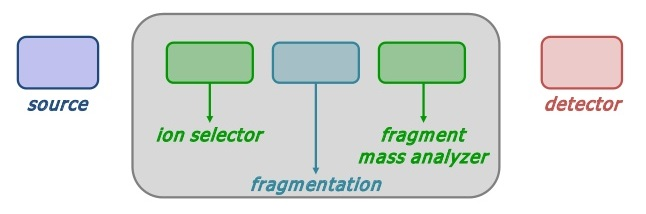
\includegraphics[width=\textwidth]{tandem_ms}
\caption[MS/MS schema]{Illustration of the tandem MS workflow. The first spectrometer acts as an ion selector, that not only registers spectra, but also lets through ions with a given \ac{m/z} ratio. The second spectrometer does not perform mass analysis, but instead provides the medium where peptide fragmentation (see section \ref{subsec:fragmentation}) occurs. Finally the third spectrometer records fragment mass spectra. Taken from \href{https://www.slideshare.net/joachimjacob/bits-introduction-to-mass-spec-data-generation}{https://www.slideshare.net/joachimjacob/bits-introduction-to-mass-spec-data-generation}.}
\label{fig:tandem_ms}
\end{figure}


\stepcounter{footnote}

Shotgun proteomics analyses make use of two or more mass spectrometers connected in series, giving rise to the so-called Tandem MS (\ac{MS/MS}) workflow. In this setting, each mass spectrometer collects a different type of spectra and thus different information (see figure \ref{fig:shotgun}). An extra spectrometer, usually a quadrupole, is introduced in between.

\begin{itemize}

\item The first spectrometer records the intensity versus \ac{m/z} ratio of the peptides eluting from the column at a given time and is used to filter ions exhibiting a selected \ac{m/z} ratio (in the \ac{DDA} protocol).

\item The ions (ionized peptides) filtered in the first spectrometer undergo fragmentation in the second spectrometer. %, as explained in \ref{subsec:fragmentation}.

\item The last spectrometer records the intensity versus \ac{m/z} ratio of the fragments produced in the previous step. The resulting spectrum can be use to read out the peptide sequence.

\end{itemize}

\begin{figure}[!h]
\centering
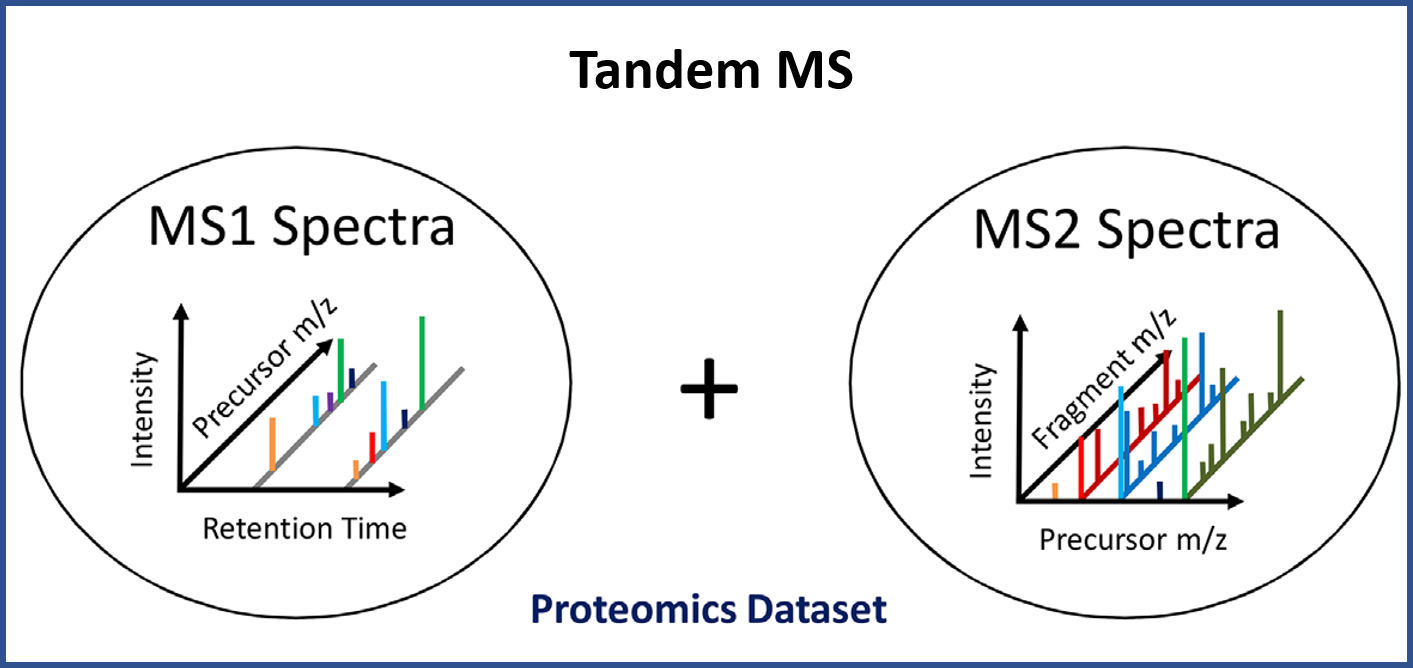
\includegraphics[width=\textwidth]{shotgun_adapted}
\caption[MS/MS spectra]{Illustration of the different spectra collected in tandem MS. MS1 spectra record precursor intensity vs \ac{m/z} ratio at different times. MS2 spectra record the same magnitudes but the signal is generated by the fragments produced during fragmentation by the ion filtered in the first spectrometer. Altogether, they enable peptide identifications. Figure adapted from \cite{Verheggen2017}.}
\label{fig:shotgun}
\end{figure}

\subsection{Fragmentation}
\label{subsec:fragmentation}

Fragmentation occurs in the second spectrometer. What is it, and why is it done? The information that can be extracted from \ac{MS1} outputs consists of the \ac{m/z} ratio and retention time of the peptide ion, but not its sequence. Having the latter is paramount if the spectrum is to be matched to a theoretical peptide. Fortunately, the peptide sequence of the ions can be inferred when fragmentation is performed.

\begin{figure}[!h]
\centering
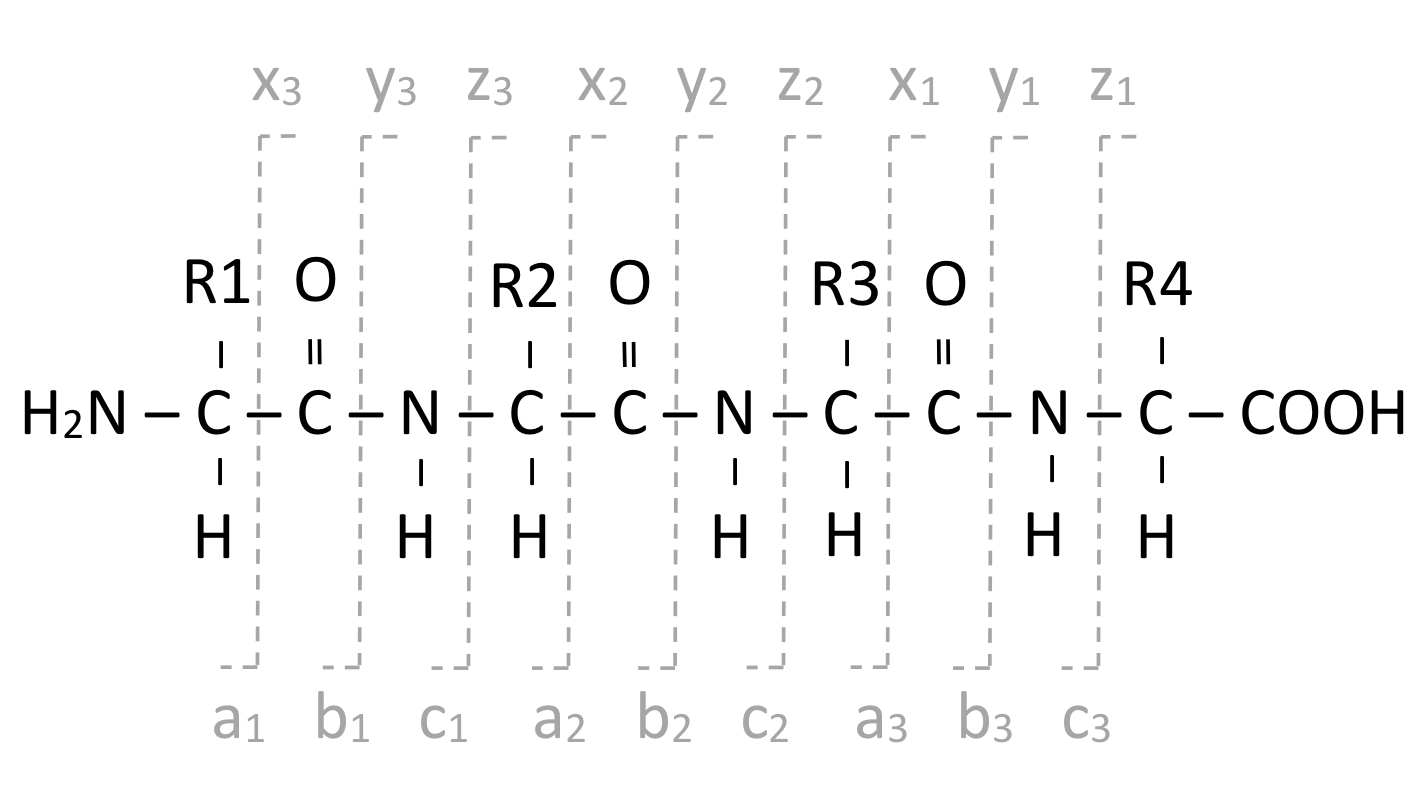
\includegraphics[width=0.8\textwidth]{abcxyz}
\caption[Fragment ions nomenclature]{\textbf{Fragment ions nomenclature}. The common fragments and their relation to the peptide sequence can be organized into 2 groups of 3 series each. The abc fragments keep the N-terminal residue, while xyz keep the C-terminal one. Specific fragmentation techniques make fragments belonging to one series more likely than others. Other fragments are possible but much less likely. The fragment nomenclature was introduced in \cite{Roepstorff1984}.}
\label{fig:abcxyz}
\end{figure}


During peptide fragmentation, bonds along the peptidic chain are broken, turning the peptide into smaller fragments. These fragments will consist of truncated versions of the original peptide at different positions, thus making it possible to read an \ac{m/z} ratio difference between any pair of fragment ions \cite{Barsnes2008}. The difference can be exploited to deduce which aminoacid makes up for that difference. If this process is repeated for enough pairs of contiguous fragments, with the right software, a sequence can be read from the \ac{MS/MS} spectrum, as  explained in section \ref{sec:search_engines}.

%A given bond will be more likely to break the less stable it is. This makes (I) the \ce{C_$\alpha$}-\ce{CO}, (II) the peptidic \ce{CO}-\ce{NH}, and (III) the \ce{C_$\alpha$}-\ce{NH} bonds the most likely to break (see figure \ref{fig:abcxyz}). A nomenclature REF was introduced to name these fragments:



%%PAG 123 COMPUTATIONAL METHODS
%Fragmentation in proteomics is performed via (I) collision-induced (CID) or (II) electron-induced (EID) dissociation. CID is an ergodic fragmentation technique where peptides enter a collision cell containing an inert gas. Given enough kinetic energy, hits between ionized peptides and the gas will trigger the fragmentation of the peptide into smaller units. \cite{Barsnes2008}. Since the kinetic energy is randomly distributed across the peptide, the weakest bonds will break first. This results in the production of mostly b and y fragments, as well as the loss of any chemical modifications \cite{Barsnes2008}.
%
%%CITE pag 134 computational methods
%
%EID is produced by the hits against the molecule, which tend to occur on the areas of the peptide more positively charged. Thus, the fragmentation process is not ergodic and returns TYPE ions. More importantly, chemical modifications are not lost in the process.
 
\section{Spectra processing: search engines}
\label{sec:search_engines}

Computational analysis of MS data starts with the matching of the spectra to a reference proteome (see figure \ref{fig:computational_analysis}). \ac{MS} search engines are capable of performing the crucial step of peptide to spectrum matching (PSM). During this step, search engines attempt to match each observed spectrum to theoretical spectra based on the reference proteome. Theoretical spectra are obtained via (I) \textit{in silico} simulation of the spectra produced by the peptides contained in the proteome, in turn obtained by performing a virtual cleavage of the sequences in the proteome, or (II) spectral libraries, consisting of annotated observed spectra \cite{Li2012}.


\begin{figure}[!h]
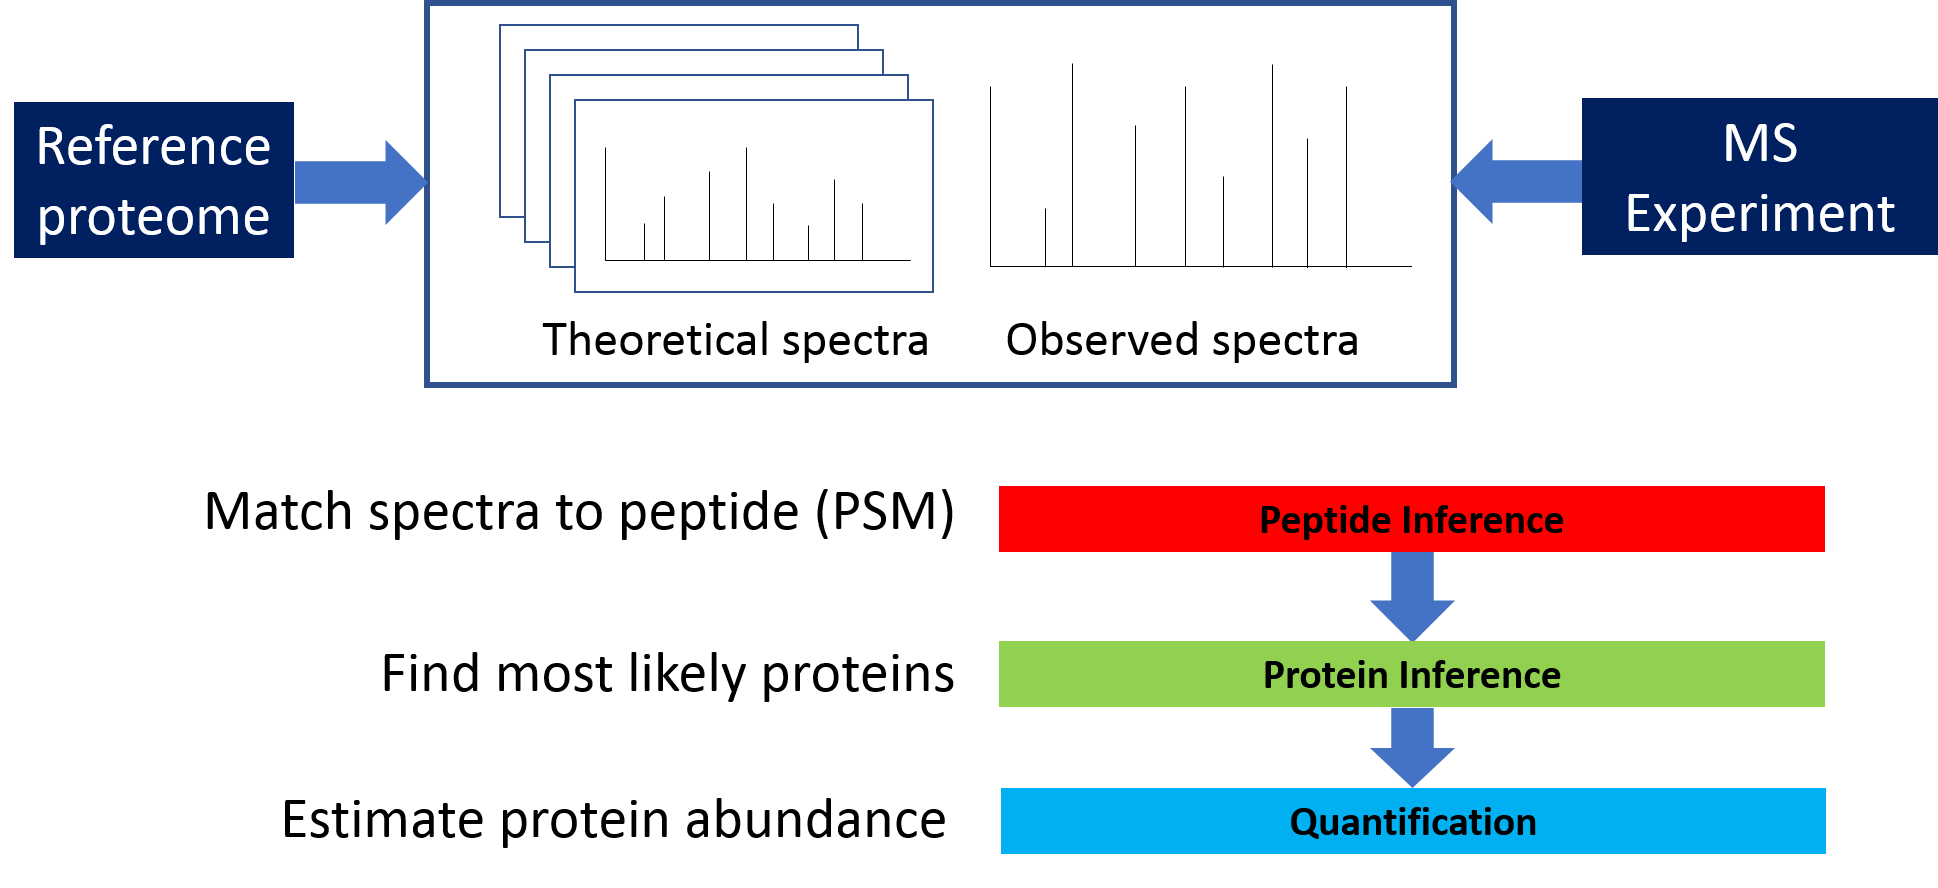
\includegraphics[width=\textwidth]{computational_analysis}
\caption[Mass spectrometry computational analysis]{Diagram of the MS computational analysis. The PSM process maps the observed spectra to a list of peptides in the reference proteome that could have generated them. In other words, the software infers what peptides were introduced in the spectrometer. The analysis continues during protein inference and quantification.}
\label{fig:computational_analysis}
\end{figure}

%\begin{figure}[!h]
%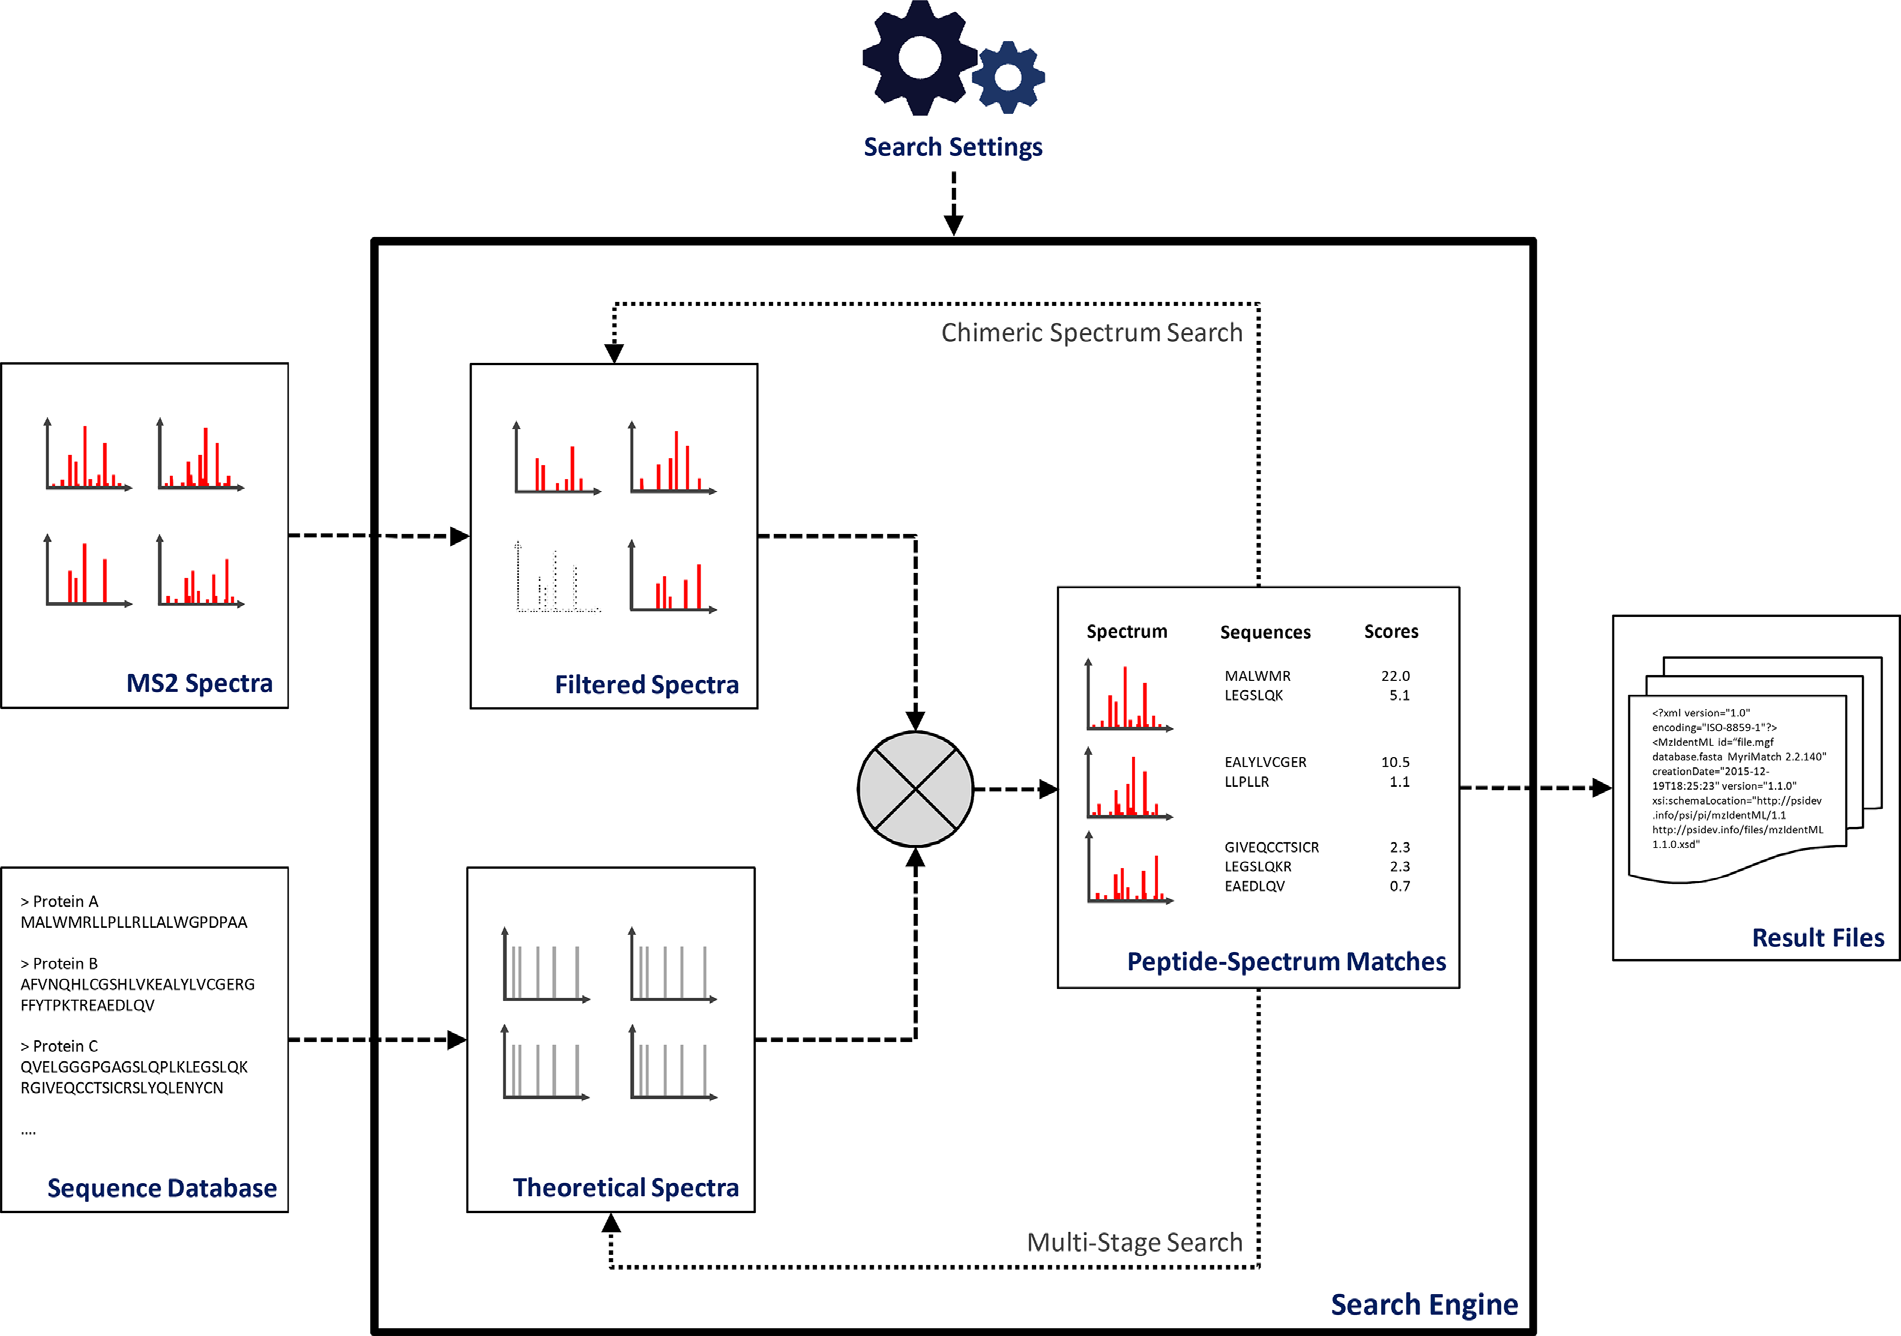
\includegraphics[width=\textwidth]{PSM}
%\caption{}
%\label{fig:PSM}
%\end{figure}

Given the stochastic nature of the protein cleavage and spectra recording processes, the resulting data exhibit variability manifested in both missing and spurious peaks \cite{Stein1999}. Furthermore, random (wrong) matches can be returned by the PSM process when running against a sufficiently big database. This translates to the generation of multiple matches for a single spectrum, of which one, if any, will be correct. Therefore, the lists of matches needs to be somehow ranked by goodness-of-fit. This issue is addressed by search engines through the deployment of statistical models that provide scoring systems. Assuming the correct protein is present in the database, a good scoring system should give the best score to the right peptide. Under this circumstances, if repeated for several peptides, enough evidence for the presence of individual proteins can be collected.

Multiple search engines exist that implement different matching and scoring algorithms. The most modern ones include MS-GF+ \cite{Kim2014}, MS-Amanda \cite{Dorfer2014}, Comet \cite{Eng2013} and Andromeda \cite{Cox2011}. Notably, the results of each individual search engine can be combined to gather their strengths, at the expense of an increased computational cost and time \cite{Shteynberg2013}.



\section{Validation and quality control}
\label{sec:validation}

The scoring systems implemented in search engines provide the best matches, but they are bound to contain false identifications. Nevertheless, these scores can be used to apply a filter that aims at minimizing the amount of errors.

A common filter is the false discovery rate (FDR), usually set to 1\%, indicating that after its application, only one out of a hundred filtered matches are expected to be false positives (wrong matches).

The most commonly used method to compute the \ac{FDR} of a list of matches is the target-decoy search. Using this method, the search engine replicates the matching process, using the same spectra, but instead against a decoy database i.e it simulates random matches. The decoy database is generated by reversing, or more generally, by applying a randomization technique upon the sequences present in the original (target) database \cite{Elias2010}. 

All matches to the decoy are by definition wrong. Since the basic properties of the decoy (size, composition, etc) remain identical to those of the target, the amount of matches to the decoy exhibiting more than a given score $s$ can be regarded as an estimate of the number of false identifications ($\hat{n}_{fp}$) in the list of target results exhibiting at least the same score (see equation \ref{eq:fdr}). This is because the existence of shared properties entails that random matches are equally likely to happen in both databases \cite{Elias2010}. Together with the number of PSMs passing a given score in the target ($n_{tp} + n_{tp}$), the FDR can be computed using equation \ref{eq:fdr}.

\begin{equation}\label{eq:fdr}
FDR = \frac{\hat{n}_{fp}}{n_{fp} + n_{tp}}
\end{equation}

Equation \ref{eq:fdr} tells us that the FDR at any score $s$ can be computed by counting how many decoy hits have a score greater than $s$ ($\hat{n}_{fp}$), and dividing by the length of our target hits list. Thus, the score that makes the FDR equal to a predefined value, frequently 0.01 or 1 \%, can be computed and used as threshold for the target hits.

\begin{figure}[!h]
\centering
%\begin{subfigure}{.45\textwidth}
%    \caption*{A}
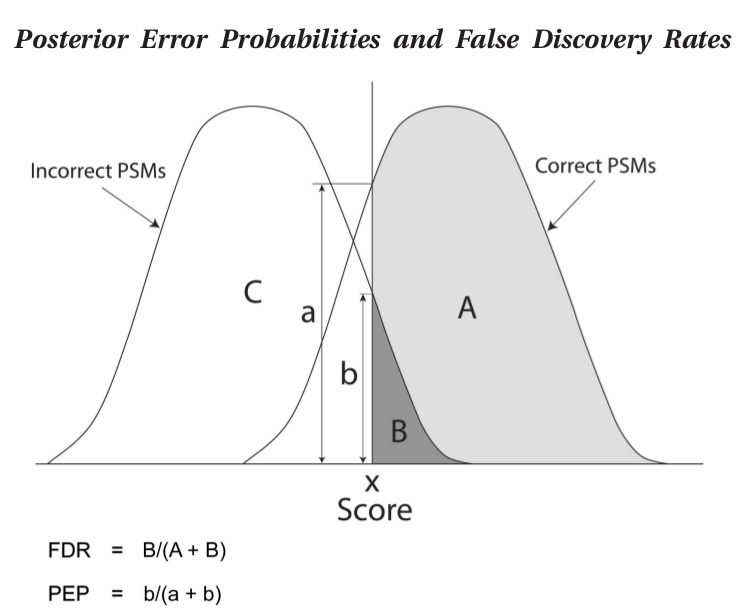
\includegraphics[width=0.9\linewidth]{pep}
\caption[FDR and PEP]{Visualizing FDR and PEP. The FDR at a given score \textit{s} is defined as the ratio between False Positives and the sum of True and False Positives found in the list of PSMs of score greater than \textit{s}. The PEP corresponds to the same ratio, but only at a specific score, hence its alternative name of local-FDR. Figure from \cite{Kall2008}.}
\label{fig:pep}
\end{figure}


The minimal FDR at which a given PSM is considered a valid match constitutes the PSM\textquotesingle s q-value, i.e. it is the smallest FDR we can allow while still keeping the PSM \cite{Nesvizhskii2010}. Related to the q-value, the Posterior Error Probability (PEP) is an estimate of the probability of a given PSM of being an incorrect assignment (see figure \ref{fig:pep}). The PSM\textquotesingle s confidence is just defined as $1-PEP$ \cite{Nesvizhskii2010}. PEP can be computed from the decoy search results and provides another useful measurement of the uncertainty in the target results.




\section{Peptide and protein inference}
\label{sec:inference}

Two steps in protein identification can be distinguished:

\begin{enumerate}

\item \textbf{Peptide inference}: infer the peptides present in the sample.
\item \textbf{Protein inference \textit{proper}}: based on the inferred peptides, infer what proteins generated them. This is not trivial as peptides are degenerate and frequently map to more than one protein \cite{Li2012}.
\end{enumerate}

The result of the PSM step returns an inferred list of peptides. The ensemble of proteins most likely to have generated the list of peptides stemming from the filtered PSMs can be identified using different algorithms \cite{Li2012} \cite{Huang2012}. Protein inference algorithms aim at explaining the maximum amount of peptides using the least amount of proteins.

\section{Protein quantification}
\label{sec:quantification}

The combination of all the aforementioned computational analyses yields a list of protein identities that reports the protein composition i.e qualitative information of the original sample. However, in most proteomics applications, quantitative data can be of great interest, as many biological phenomena are manifested mainly through changes in the protein abundances, cell compartments, rather than the simple dichotomy of the protein\textquotesingle s existence \cite{Barsnes2008}. For instance, cancer cells in response to a drug could modulate the abundance of several proteins without removing them from the cytosol or introducing new ones.

Protein quantification pipelines can be classified based on whether isobaric labelling was used (label-based) or not (label-free). These are explained in subsection \ref{subsec:labelling}. If the label-free approach is employed, more distinctions can be made based on:

\begin{itemize}
\item The proxy used for quantification: spectral counting (\ac{SC}) or extracted ion currents (\ac{XIC}). These are explained in \ref{subsec:scvsxic}


\item The way the data are brought to the protein level from the peptide level: summarization-based vs. peptide-based, explained in \ref{subsec:peptide_model}.
\end{itemize}

\subsection{Label-based and label-free approaches}
\label{subsec:labelling}

%CITE PAGE 237 COMPUTATIONAL METHODS 

Two paradigms exist in protein quantification: label-based and label-free. In label-based quantification, originally identical peptides from a number of different samples are made distinguishable by their masses via the incorporation of a label. All label-based methods simultaneously analyze several samples in each experiment, removing the difficulties associated with between-run variability \cite{Barsnes2008}. The finite number of "plexes" available for a given label sets the limit to how many samples can be differentially quantified \cite{Cox2014}. Different techniques, like Stable Isotope Labeling by Amino acids in Cell culture (SILAC) or Isotope-Coded Affinity Tags (ICAT), differ in the nature of the label and the way it is introduced. Most of them have potential limitations \cite{Patel2009}. This, together with the limited amount of samples that can be compared makes a case for label-free quantification.

In the label-free quantification approach, peptides from different samples are not labelled differently and are thus distinguished by their presence in different, independent \ac{MS} runs \cite{Barsnes2008}. In order to account for the introduced inter-run variability in peptide identifications and \ac{RT}, a match-between-runs (MBR) processing step can be carried out (see figure \ref{figure:moff_mbr}). 


\begin{figure}[!h]
\centering
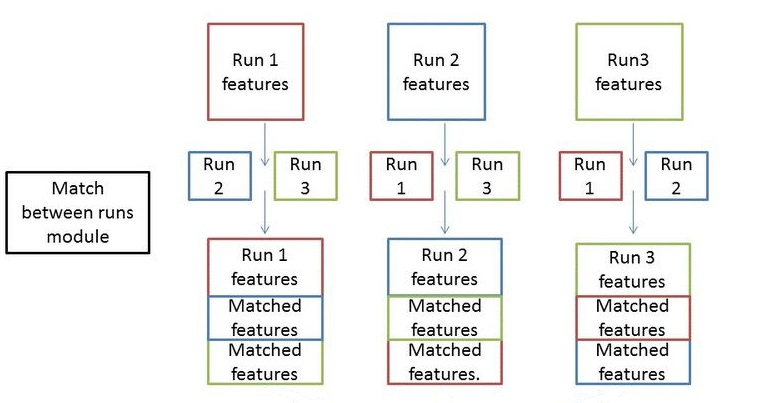
\includegraphics[width=0.9\linewidth]{mbr_workflow}
\caption[Match Between Runs module]{\textbf{\ac{MBR} step}. The information gathered from matches in replicate runs is put to use during a reanalysis of the spectra. Modified from supplementary information in \cite{Argentini2016}.}
\label{figure:moff_mbr}
\end{figure}

This way, extra identifications are attained through a reanalysis of the spectra, factoring in the information collected in replicate runs. The RT and precursor mass of unidentified spectra in one replicate is matched to that of identified spectra in the remaining replicates. As a consequence, more identifications with a lesser fraction of missing datapoints are achieved.


\subsection{SC and XIC based quantification}
\label{subsec:scvsxic}


Quantification can be spectrum counting (\ac{SC}) or extracted ion currents (\ac{XIC}) based.

On the one hand, spectrum counting based quantification is the simplest method in proteomics. The number of times a peptide is detected in the spectrometer is used as proxy for its abundance. It relies on the rationale that highly abundant peptides will have an accordingly higher intensity and are thus more likely to trigger the acquisition of MS/MS spectra. These methods have the advantage that they are very simple to implement and don\textquotesingle t require any further data processing \cite{Barsnes2008}.

On the other hand, \ac{XIC} based methods rely on intensity measurements at any level of the \ac{MS} workflow as proxies for protein abundance. A wide range of algorithms are available to process these data and output estimates of protein abundance. All of them require an intensive preprocessing step, usually including (I) taking the $log_2$ intensity to make the distributions symmetrical and thus fit for diverse parametric tests, and (II) quantile normalization to address between-runs variability in the intensity measurements. They can be classified in the bases of which MS level is used as proxy for the protein abundances and on whether or not a summarization step is performed to aggregate peptide-level data into protein-level data, or not. 


As stated in \cite{Cox2014}, "\textit{although the abundance of proteins and the probability of their peptides being selected for \ac{MS/MS} sequencing are correlated to some extent, \ac{XIC}-based methods should clearly be superior to \ac{SC} given sufficient resolution and optimal algorithms. These advantages are most prominent for low-intensity protein/peptide species, for which a continuous intensity readout is more information-rich than discrete counts of spectra}". For this reason, only the \ac{XIC} approach will be regarded in the rest of this manuscript.  

For a more robust XIC based quantification, a feature extraction step is usually executed to extract consistent descriptors of identified peak clusters in the RT-m/z plane, as shown in figure \ref{figure:moff_apex}.

\begin{figure}[!h]
\centering
\begin{subfigure}{1\textwidth}
\centering
\caption*{A}
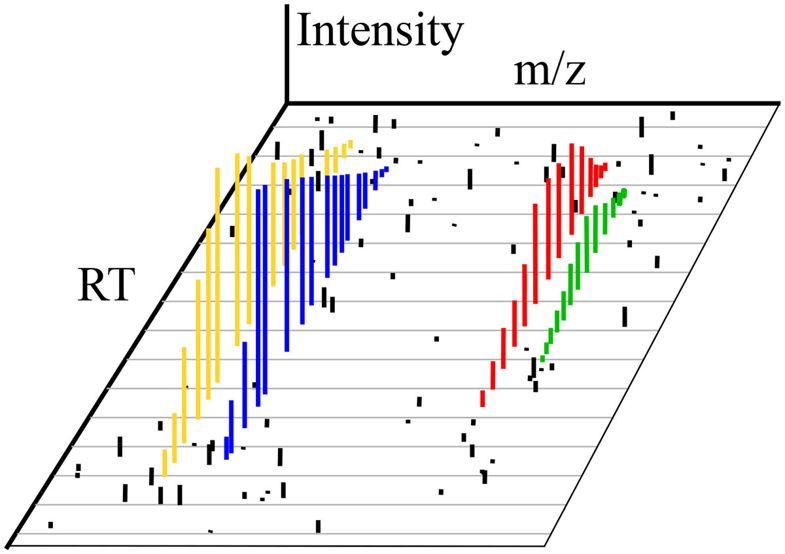
\includegraphics[width=0.7\linewidth]{apex_3d}
\end{subfigure}
\bigskip
\begin{subfigure}{1\textwidth}
\centering
\caption*{B}
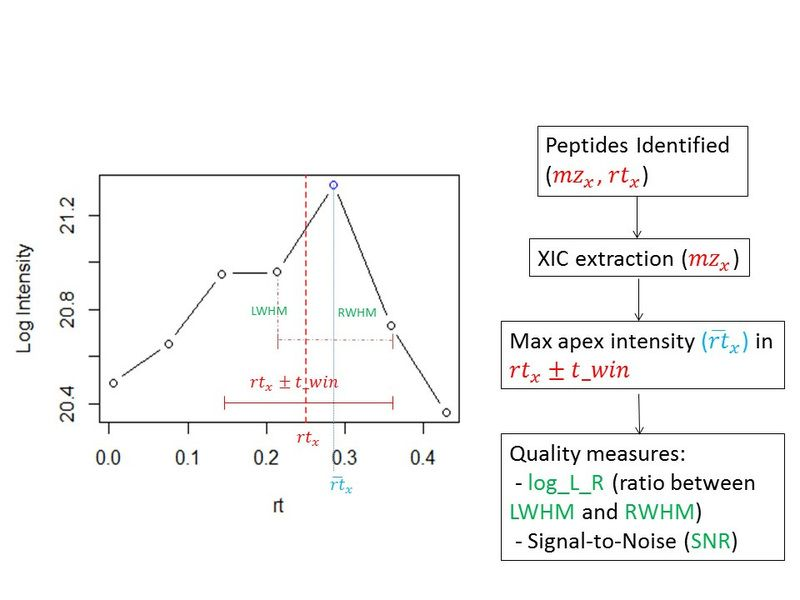
\includegraphics[width=0.7\linewidth]{apex_intensity}
\end{subfigure}
\caption[Apex MS1 intensity module]{\textbf{The apex intensity extraction step}. \textbf{A} Visualization of a 3D peak cluster on the RT / m/z plane. Ion currents are detected with varying degrees of intensity over a more or less narrow time window, spreading the signal over time. Taken from \cite{Smith2014}. \textbf{B} A refinement analysis of these data attempts to fit a mathematical model of the signal over time and extract a representative measurement, such as the highest (apex) \ac{MS1} intensity. Modified from supplementary information in \cite{Argentini2016}.}
\label{figure:moff_apex}
\end{figure}


\subsection{\ac{XIC}-peptide-based models for label-free quantification}
\label{subsec:peptide_model}

The data collected in the mass spectrometer refers to peptides originating from a latent protein composition, given by the original sample. However, the data interpretation requires the transfer of these peptide-level data into the protein level. This can be done by either (I) performing an aggregation of the peptide-level data, where a summary value of the peptide-level data is taken as representative for the protein-level data, or (II) performing the protein quantification directly at the peptide-level by means of linear regression models.

As stated in \cite{Goeminne2015} "\textit{peptides originating from the same protein can indeed be considered technical replicates and theoretically should lead to similar abundance estimates. However, the summarization of the peptide intensities into protein expression values is cumbersome, and most summarization-based methods do not correct for differences in peptide characteristics or for the between-sample differences in the number of peptides that are identified per protein. This might introduce bias and differences in uncertainty between the aggregated protein expression values, which are typically ignored in downstream data analysis steps}".

It is for this reason that peptide-based models offer the statistical framework required to learn as much from the data as possible. This translates into improved results when compared to the other aforementioned methods \cite{Goeminne2015}. %This hypothesis is the motivation for the method explained in chapter \ref{chap:model}.
